% Procedure for preparation

\stepcounter{tableCounter} % Increment counter
\setcounter{rowCounter}{0} % Reset counter
\begin{tabularx}{\textwidth}{|>{\columncolor{tableColumnColor}}c|>{\columncolor{tableColumnColor}}c|>{\columncolor{tableColumnColor}}c|>{\columncolor{tableColumnColor}}c|X|}
  \hline
  \rowcolor{tableHeaderColor}
  ID                    & CK 1      & CK 2      & CK 3      & Description \\ \hline

  \arabic{tableCounter} & \checkbox & \checkbox & \checkbox &
  \begin{minipage}[t]{\linewidth}
    \textbf{Software Preparation}
    \vspace{1mm} % Just slightly add vspace to prevent clipping into table border
  \end{minipage}
  \\ \hline

  \procedureItem{
    \hl{
      Install System according to
    }
  \\
    \hl{
      PRO\_OP\_DACS\_004\_Installation-Control\_01
    }
  \\
    \hl{
      Do not launch yet (do not run start\_maria\_test)
    }
  }

  \procedureItem{

    \hl{Check config files (08\_DACS\textbackslash01\_Software\textbackslash07\_Configuration, especially}

    \begin{itemize}
      \item \hl{Update firing parameter specification}
      \item \hl{Choose sequence and update activation times}
      \item \hl{Update sensor thresholds}
    \end{itemize}

  }

  \procedureItem{
    Make sure the following files are downloaded from Sharepoint (08\_DACS\textbackslash01\_Software\textbackslash07\_Configuration) and saved to:
    \begin{itemize}
      \item /home/dacs/git/configuration\_tests/
            \\
            PRO\_DACS\_Configuration
      \item /home/dacs/git/software-rpi4/state\_machine/src/
            \\
            state\_machine\_list.csv

      \item /home/dacs/git/software-rpi4/state\_machine/src/
            \\
            state\_machine\_sequences.csv

      \item /home/dacs/git/software-rpi4/throttling\_control/src/
            \\
            setpoint\_publisher.py

      \item /home/dacs/git/software-rpi4/throttling\_control/src/
            \\
            control.py
    \end{itemize}
  }

  \stepcounter{tableCounter}
  \setcounter{rowCounter}{0} % Reset counter

  \arabic{tableCounter} & \checkbox & \checkbox & \checkbox &
  \begin{minipage}[t]{\linewidth}
    \textbf{Launch System}
    \vspace{1mm} % Just slightly add vspace to prevent clipping into table border
  \end{minipage}
  \\ \hline

  \procedureItem{
    \hl{Launch System according to}
  \\
    \hl{PRO\_OP\_DACS\_004\_Installation-Control\_01}
  }

  \stepcounter{tableCounter}
  \setcounter{rowCounter}{0} % Reset counter

  \arabic{tableCounter} & \checkbox & \checkbox & \checkbox &
  \begin{minipage}[t]{\linewidth}
    \textbf{Test System}
    \vspace{1mm} % Just slightly add vspace to prevent clipping into table border
  \end{minipage}
  \\ \hline

  \procedureItem{
    \hl{
      In the UI test the sequence of phases by going through them and check if the right actuators are controllable.
      Trigger the sequences in Ignition and Firing phase (if control valves positions are changed during firing also check that the setpoint curve is right).
      After that check the abort sequences by pressing ‘Ctrl-Space’ once in Fuel Filling, Oxidizer Filling and Firing
    }
  }

  \procedureItem{
    \hl{
      Check the abort sequences by pressing ‘Ctrl-Space’ once in Fuel Filling, Oxidizer Filling and Firing
    }
  }
  \procedureItem{
    \hl{
      With another person observing the valves or the Relay lights in the DACS compartment, check that immediately after toggling the switch in the UI the actuator is activated
    }
  }

  \procedureItem{
    \hl{
      Check the functionaltity of the manual override box the status lights on the trailer by switching through all circuits
    }
  }

  \procedureItem{
    Check that plotjuggler plots keep up with the sensor values (let it run for 3-5 minutes)
  }

  \procedureItem{
    Check that the UI keeps up with the sensor values:
    \begin{itemize}
      \item \texttt{cd catkin\_ws}
      \item \texttt{source ./devel/setup.bash}
      \item \texttt{rostopic echo /sensor\_prg\_p}
    \end{itemize}


    Compare whether rostopic echo measurement values change simultaneously with UI, also the cursor should not lag in the UI

    In case of system delays:
  \\
    \texttt{/home/dacs/git/software-rpi4/data\_acquisition/src/core/T7(\_streaming).py}
  \\
    and in
    \texttt{translate\_data\_2\_ros} change \texttt{j = j \% 40} to a higher number and restart
  }

  \procedureItem{
    Ensure that the rosbags are being saved in catkin\_ws/src/rosbags

    However, after checking delete them again
  }

  \procedureItem{
    Press Ctrl-C in all running Terminal windows, make sure all changes are saved, then close all windows and shut down PCs
  }


  \stepcounter{tableCounter}
  \setcounter{rowCounter}{0} % Reset counter

  \arabic{tableCounter} & \checkbox & \checkbox & \checkbox &
  \begin{minipage}[t]{\linewidth}
    \textbf{Packing}
    \vspace{1mm} % Just slightly add vspace to prevent clipping into table border
  \end{minipage}
  \\ \hline

  \procedureItem{
    Assemble the hardware as mentioned in sections B and C
  }

  \procedureItem{
    \hl{
      Place the three monitors with foil to protect the displays in the two big DACS boxes
    }
  }

  \procedureItem{
    \hl{
      Put PC power cables, power strips, DP cables, mouses, keyboards and manual override box in the same boxes
    }
  \\
    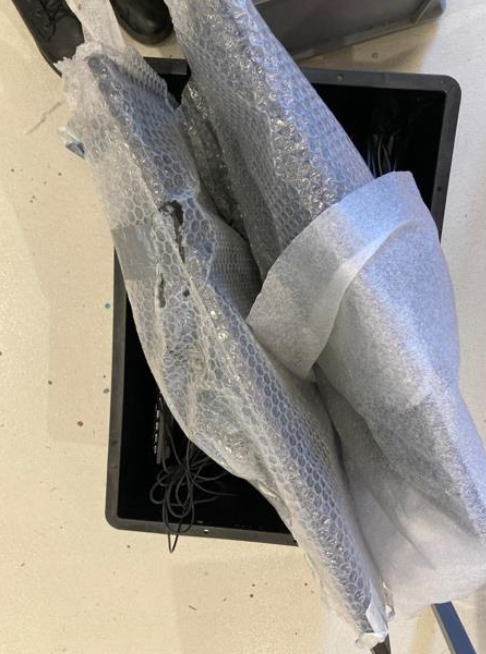
\includegraphics[width=0.5\textwidth]{assets/monitors-in-box.png}
  }

  \procedureItem{
    DACS Box 1 with Monitor 1 \& 2, corresponding keyboard and mouse, 3 DP cables, and 3 monitor power cables
  \\
    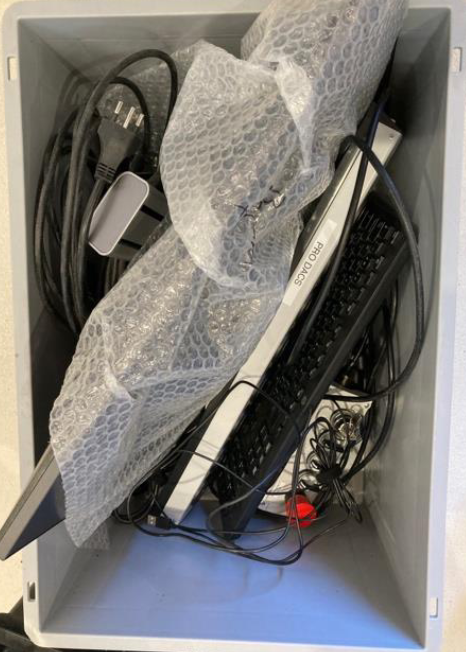
\includegraphics[width=0.5\textwidth]{assets/other-monitor-in-box.png}
  \\
    DACS Box 2 with Surveillance/KiDAQ Monitor, corresponding keyboard and mouse 2 PC power adapters, manual override box, 2 power strips, extension cable
  }

  \procedureItem{
    \hl{
      Put the two PCs in the smaller DACS box together with the Ethernet switch, Ethernet cables and Switch‘s power cable
    }
  \\
    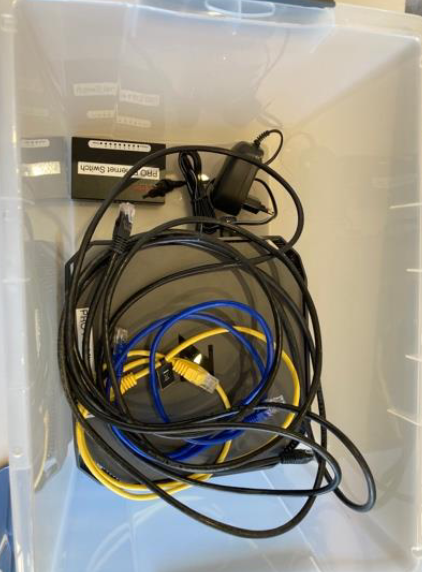
\includegraphics[width=0.5\textwidth]{assets/smaller-dacs-box.png}
  \\
    \hl{
      Smaller DACS box with 2 PCs, Ethernet Switch, Ethernet Switch power cable, 2 short Ethernet cables, replacment Etheret cable
    }
  }
\end{tabularx}
